\begin{frame}[fragile]{Visualização da representação por lista de arestas}

    \begin{figure}
        \centering

        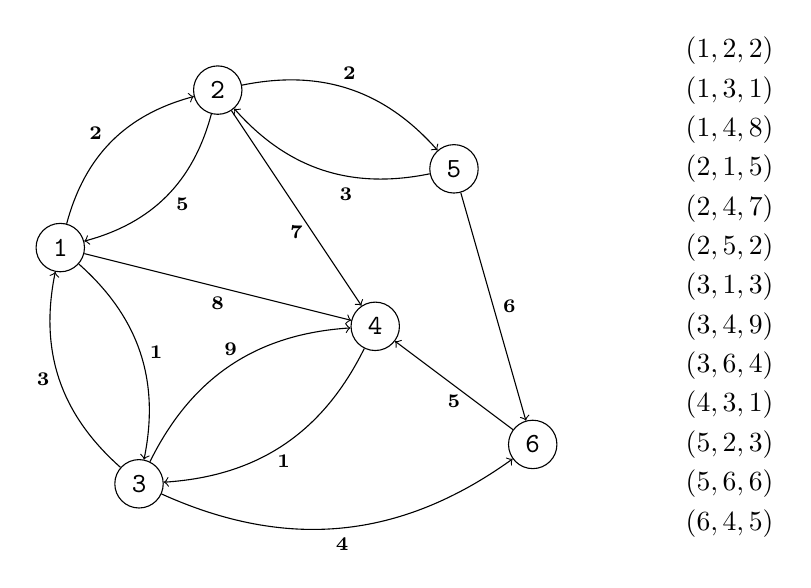
\begin{tikzpicture}
            \node[draw,circle] (A) at (0, 3) { \tt 1 };
            \node[draw,circle] (B) at (2, 5) { \tt 2 };
            \node[draw,circle] (C) at (1, 0) { \tt 3 };
            \node[draw,circle] (D) at (4, 2) { \tt 4 };
            \node[draw,circle] (E) at (5, 4) { \tt 5 };
            \node[draw,circle] (F) at (6, 0.5) { \tt 6 };

            \draw[->] (A) to [bend left] node[anchor=east,yshift=0.1cm] { \scriptsize $\mathbf{2}$ } (B);
            \draw[->] (B) to [bend left] node[anchor=west,yshift=-0.1cm] { \scriptsize $\mathbf{5}$ } (A);
            \draw[->] (A) to [bend left] node[anchor=west] { \scriptsize $\mathbf{1}$ } (C);
            \draw[->] (C) to [bend left] node[anchor=east] { \scriptsize $\mathbf{3}$ } (A);
            \draw[->] (D) to [bend left] node[anchor=north] { \scriptsize $\mathbf{1}$ } (C);
            \draw[->] (C) to [bend left] node[anchor=south] { \scriptsize $\mathbf{9}$ } (D);
            \draw[->] (B) to [bend left] node[anchor=south] { \scriptsize $\mathbf{2}$ } (E);
            \draw[->] (E) to [bend left] node[anchor=north,xshift=0.3cm,yshift=-0.1cm] { \scriptsize $\mathbf{3}$ } (B);

            \draw[->] (A) -- node[anchor=north] { \scriptsize $\mathbf{8}$ } (D);
            \draw[->] (B) -- node[anchor=north,yshift=-0.1cm] { \scriptsize $\mathbf{7}$ } (D);
            \draw[->] (C) to [bend right] node[anchor=north] { \scriptsize $\mathbf{4}$ } (F);
            \draw[<-] (D) -- node[anchor=north] { \scriptsize $\mathbf{5}$ } (F);
            \draw[->] (E) -- node[anchor=west] { \scriptsize $\mathbf{6}$ } (F);

            \node at (8.5, 5.5) { $(1, 2, 2)$ };
            \node at (8.5, 5) { $(1, 3, 1)$ };
            \node at (8.5, 4.5) { $(1, 4, 8)$ };
            \node at (8.5, 4) { $(2, 1, 5)$ };
            \node at (8.5, 3.5) { $(2, 4, 7)$ };
            \node at (8.5, 3) { $(2, 5, 2)$ };
            \node at (8.5, 2.5) { $(3, 1, 3)$ };
            \node at (8.5, 2) { $(3, 4, 9)$ };
            \node at (8.5, 1.5) { $(3, 6, 4)$ };
            \node at (8.5, 1) { $(4, 3, 1)$ };
            \node at (8.5, 0.5) { $(5, 2, 3)$ };
            \node at (8.5, 0) { $(5, 6, 6)$ };
            \node at (8.5, -0.5) { $(6, 4, 5)$ };
        \end{tikzpicture}

    \end{figure}

\end{frame}
